% !Mode:: "TeX:UTF-8"
% !TEX program  = xelatex

\documentclass{cumcmthesis}
%\documentclass[withoutpreface,bwprint]{cumcmthesis} %去掉封面与编号页
\usepackage[framemethod=TikZ]{mdframed}
\usepackage{url}   % 网页链接
\usepackage{subcaption} % 子标题
\usepackage{enumitem}
\usepackage{geometry}
\usepackage{booktabs}

\geometry{left=2.5cm,right=2.5cm,top=2.5cm,bottom=2.5cm}
\title{“同心协力”策略研究}
\tihao{}
\baominghao{4321}
\schoolname{北京大学}
\membera{刘宇林}
\memberb{蒋衍}
\memberc{董婉萍}
\supervisor{}
\yearinput{2019}
\monthinput{09}
\dayinput{15}
\begin{document}

 \maketitle
 \begin{abstract}
本文根据题目的要求,对“同心协力”游戏项目的过程进行深入分析,结合实际情况,考虑了可能出现的不同条件、影响因素,在合理的抽象及假设之下,建立数学模型,确定除了游戏最优策略,从而达到连续颠球的次数尽可能多的目的。

首先从理想状态出发,假设队员的发力可以精确控制,经过对过程的受力分析及计算,我们只需要让队员提供恒力,使得每次发力后,排球获得的的能量与碰撞过程中损失的能量相等,从而排球弹跳过程稳定为周期运动,即可达到目标。

再考虑现实情形中,队员发力时机和力度不可能做到精确控制,存在一定误差,于是鼓面可能出现倾斜。通过计算,我们确定了队员的发力时机和力度与某一特定时刻的鼓面倾斜角度的关系,并制定出了相应的调整策略。对于具体的出现误差的实例,我们又相应地给出了具体的调整策略,并进一步分析在现实情形中这种调整策略的实施效果。

最后我们分析了模型的误差来源,从准确性、稳定性、适用性角度,对模型进行了评估和改进,并对模型的推广方向进行了展望,具有一定参考意义。

\keywords{刚体力学\quad  动量\quad   受力分析\quad  最优策略}
\end{abstract}

%目录  2019 明确不要目录,我觉得这个规定太好了
%\tableofcontents

%\newpage

\renewcommand\thesection{\arabic{section}}
\section{问题重述}
“同心协力”是一项团队协作能力拓展项目。该项目的道具是一面牛皮双面鼓,鼓身中间固定多根绳子,绳子在鼓身上的固定点沿圆周呈均匀分布,每根绳子长度相同。团队成员每人牵拉一根绳子,使鼓面保持水平。项目开始时,球从鼓面中心上方竖直落下,队员同心协力将球颠起,使其有节奏地在鼓面上跳动。颠球过程中,队员只能抓握绳子的末端,不能接触鼓或绳子的其他位置。

项目所用排球的质量为270g。鼓面直径为40cm,鼓身高度为22cm,鼓的质量为3.6kg。队员人数不少于8人,队员之间的最小距离不得小于60cm。项目开始时,球从鼓面中心上方40cm处竖直落下,球被颠起的高度应离开鼓面40cm以上,如果低于40cm,则项目停止。项目的目标是使得连续颠球的次数尽可能多。

我们的任务是,根据题目给出的不同条件,建立数学模型解决以下问题:
\begin{enumerate}
\item 在理想状态下,每个人都可以精确控制用力方向、时机和力度,试讨论这种情形下团队的最佳协作策略,并给出该策略下的颠球高度。
\item 在现实情形中,队员发力时机和力度不可能做到精确控制,存在一定误差,于是鼓面可能出现倾斜,建立模型描述队员的发力时机和力度与某一特定时刻的鼓面倾斜角度的关系。
\item 在现实情形中,根据问题2的模型,是否需要调整问题1中给出的最优策略?如果需要,如何调整?
\item 当鼓面发生倾斜时,球跳动方向不再竖直,于是需要队员调整拉绳策略。假设人数为10,绳长为2m,球的反弹高度为 60cm,相对于竖直方向产生1°的倾斜角度,且倾斜方向在水平面的投影指向某两位队员之间,与这两位队员的夹角之比为1:2。为了将球调整为竖直状态弹跳,请给出在可精确控制条件下所有队员的发力时机及力度,并分析在现实情形中这种调整策略的实施效果。
\end{enumerate}

\section{问题分析}
图x给出了题述情境的几何示意图,上方圆球为排球,下方圆柱体为同心鼓,四周发出的射线为各队员手中控制的绳子。当队员们松开绳子时,...用力拉紧绳子时,...。初始排球从空中自由下落,与鼓面碰撞时弹起...游戏的目标即使排球弹起方向尽量平稳,每次弹起高度都超过40cm。

此系统的理想状态是排球和鼓都恰在竖直方向作周期运动,每次弹起高度相同,如若每名队员都能精确控制用力方向、时机与力度,不难找到一组使系统保持平稳周期运动的参数。但现实中难以做到精确控制,从而会发生弹起高度不足或球轨迹歪斜掉出鼓面,导致游戏失败。本文旨在...其中第一部分,第二部分...

\section{符号约定}
\begin{longtable}[c]{cc}
%begin{table}[htbp!]
    %\centering
    \caption{符号使用与说明}\label{tab:001}\\
        \toprule[1.5pt] 符号 & 含义\\ \hline \hline \endfirsthead %1第一页表头
        \toprule[1.5pt]  符号 & 含义\\ \hline  \hline \endhead %2续页表头
        $M$ & 鼓的质量\\
        \hline
        $m$ & 排球的质量\\
        \hline
        $r$ & 鼓的半径\\
        \hline
        $l$ & 绳子的长度\\
        \hline
        $h$ & 鼓质心的高度\\
        \hline
        $d$ & 鼓与球相碰时鼓的位移\\
        \hline
        ${F}$ & 人拉绳子的力\\
        \hline
        $T$ & 排球弹起落下一个周期的时长\\
        \hline
        $v_1$ & 鼓在与球碰撞前的速度\\
        \hline
        $v_1^{'}$ & 鼓在与球碰撞后的速度\\
        \hline
        $v_2$ & 球在与鼓碰撞前的速度\\
        \hline
        $v_2^{'}$ & 球在与鼓碰撞后的速度\\
        \hline
        $\overrightarrow{L}$ & 鼓的角动量\\
        \hline
        $\theta$ & 绳与竖直方向的夹角\\
        \hline
        $\overrightarrow{\omega}$ & 鼓的角速度\\
        \hline
        $I$ & 鼓的转动惯量\\
        \bottomrule[1.5pt]
%\end{table}
\end{longtable}

\section{模型假设}

\begin{enumerate}
	\item 绳子的劲度系数极大,不考虑其长度变化;
	\item 所有人握绳端处的高度相同;
	\item 鼓和排球都可视为刚体,自身不发生形变;
	\item 不考虑风与空气阻力的一切影响;
	\item 不考虑排球自身的旋转;
	\item 排球与鼓面碰撞时不在鼓面滑动;
	\item 所有碰撞都符合牛顿碰撞定律,且都在瞬间完成.
%	\item 在问题2求解中:
%	\begin{itemize}
%		\item 假设鼓在水平方向上没有运动,这是为了方便在分析时锁定绳子上的力和方向。为说明该假设的科学性,我们先计算在鼓保持静止在最低点时绳子上的拉力。即:
%		\begin{equation*}
%			8Fcos \theta  \geq Mg
%		\end{equation*}
%		可以解出绳子上有拉力70N。本问中,在某一方向的最大拉力为90N,此时有位移:
%		\begin{equation*}
%			\frac{ \Delta Fsin \theta} {2M} t^{2}
%		\end{equation*}
%		\item 假设在每一个时间段(0.1s)内设角速度是不变的。下给出说明:
%
%		首先根据刚体转动公式有
%		\begin{equation*}
%			\sum  \overrightarrow{F} \times   \overrightarrow{r} =  \overrightarrow{L}
%		\end{equation*}
%		\begin{equation*}
%			\overrightarrow{L} = I\overrightarrow{ \omega }
%		\end{equation*}
%		$\overrightarrow{F}$的作用时间为0.1s,在这一过程中,$\overrightarrow{F}$的方向变化不大,而$\overrightarrow{L}$方向永远与$\overrightarrow{F}$垂直,模被重心到$\overrightarrow{F}$的距离唯一决定,故做外积后$\overrightarrow{L}$的模可以视为不随$t$改变,方向也不随$t$改变,从而$\overrightarrow{\omega}$可视为在0.1s内不变,所求角度为:
%		\begin{equation*}\label{eq:eps}
%			\theta =  \frac{\overrightarrow{ L_{0} }}{I} t
%		\end{equation*}
%	\end{itemize}
%	\item \ldots
\end{enumerate}

\section{模型建立与求解}
以鼓质心所在竖直线上与手握处平齐为原点,以过鼓质心且与鼓面平行的任一直线及其水平面上的垂线为x,y轴、竖直方向为z轴,建立空间直角坐标系如图...。

\subsection{精确控制下的运动模型}
初始时排球从40cm高空静止落下,排球与鼓各自在z轴方向作周期运动。为消除不确定因素使排球与鼓保持平稳的周期运动,在此设定二者运动周期相同,排球每次弹起高度都为40cm,每个周期球与鼓碰撞一次,碰撞点为$(0,0,0)$.
\subsubsection{排球的运动模型}
在我们设定的条件下,排球每次弹起达到相同高度,故需每次与鼓面碰撞后都有相同的初速度,且与碰撞前速度等大反向,撞后仅受重力作用,故有:$$v_2^{'}=v_2$$ $$\frac{1}{2}g(\frac{T}{2})^2=0.4$$
其中$v_1, v_2, v_1^{'}, v_2^{'}$均取沿z轴向上为正,向下为负。所有符号代表的值均为国际制单位。
\subsubsection{鼓的运动模型}
在不与排球碰撞时,鼓仅受到各队员拉力与重力的作用。由于队员均匀站在周围,x、y方向受力相互抵消,因此仅z方向的合力为非零,鼓在z方向受力状况为:
$$Ma=nF\cos\theta-Mg$$
\subsubsection{球鼓碰撞}
假设球鼓碰撞服从牛顿碰撞定律,法向相对速度在碰撞前与碰撞后比值恒定:
$$e=\frac{|v_2^{'}-v_1^{'}|}{|v_2-v_1|}$$
其中$e$为碰撞系数,只与碰撞物体材质有关而与碰撞速度无关。查阅资料估计球与鼓面的碰撞系数$e=0.9$.
\subsubsection{模型求解}
由排球弹起最高点为40cm不难解出运动周期与排球和鼓的撞前、撞后速度:
\begin{equation*}
\left\{
\begin{array}{lr}
T = 0.5714 \\
v_2 = -2.8 \\
v_2^{'} = 2.8 \\
v_1 = 0.3684 \\
v_1^{'} = -0.0514
\end{array}
\right.
\end{equation*}
因此队员们需要控制用力时机与大小,使得鼓在一个周期T内走过的位移和量恰好为零,碰撞前后速度恰符合上述要求。为简化用力策略,不妨设鼓在周期内第一段时间$t_1$以恒定加速度$a_1$运动,在周期内第二段时间$t_2$以恒定加速度$a_2$运动,$v-t$图如图xxx所示。

\subsection{问题2}
本问主要运用刚体转动公式,先求出鼓(空心圆柱体)的转动惯量,建立空间直角坐标系并进行受力分析,最后得出转动的角度。
\subsubsection{转动惯量$I$的确定}
由于本题涉及刚体转动,因此需要先计算出转动惯量$I$,由于鼓绕轴的转动不是常见的转动模型,自然地,我们考虑用微元法解决。
\begin{description}
\item[步骤一] 如下图所示,取一垂直于转轴的剖面,得到一个矩形框,
\begin{figure}[!h]
    \centering
    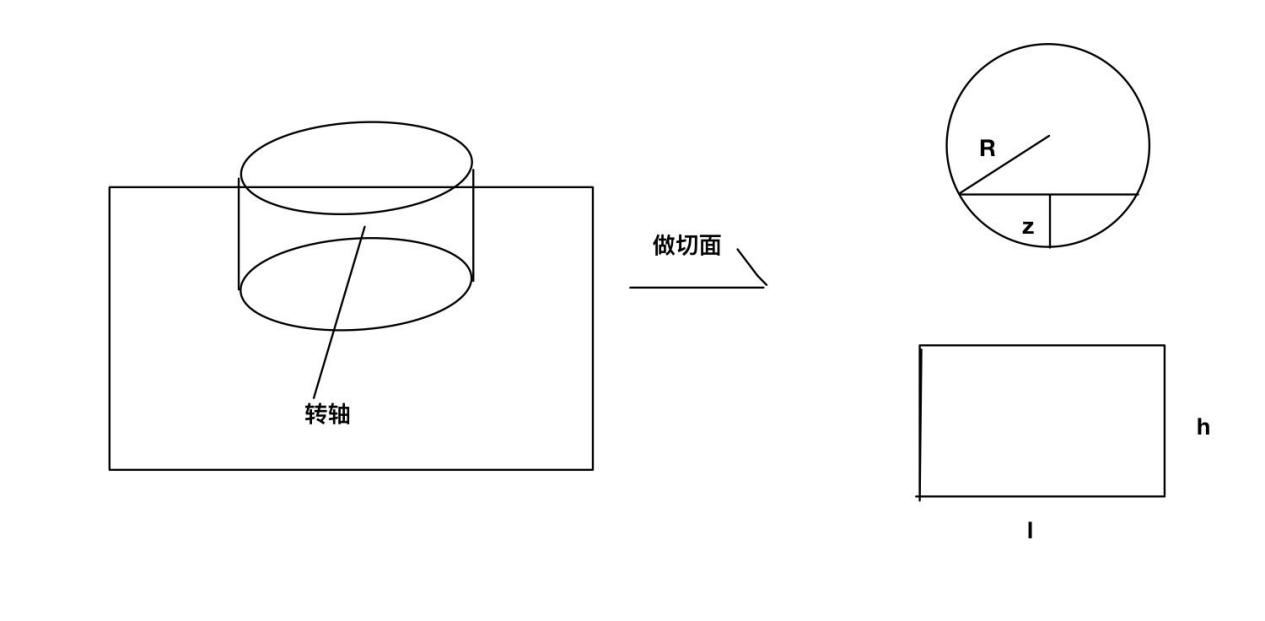
\includegraphics[width=.6\textwidth]{sectional}
    \caption{鼓的剖面图}
    \label{fig:p1}
\end{figure}
由公式
\begin{equation*}
	I =  \int r^2 dm
\end{equation*}
我们取每条矩形框为微元,考虑矩形框的转动惯量。
\item[步骤二] 求解每条矩形框的转动惯量,分解为求四条边的转动惯量,已知线段绕其中心转动的转动惯量为
\begin{equation*}
	I =  \frac{ml^2}{12}
\end{equation*}
再由转动轴定理\footnote{将转轴外移$d$,则转动惯量增加$m\cdot d \cdot d$}便可以得到每条线框的转动惯量。
\item[步骤三] 又设这些矩形框宽度为$dz$,便可以计算出他们的质量,再把$dz$从$0\~{}2r$积分便可以得到整体的转动惯量,计算公式为
\begin{equation*}
	\int_{0}^{0.4}  \frac{ m_{1} l_{1}^{2}+ 3 m_{1} l_{2}^{2} + m_{2} l_{2}^{2}+ 3m_{2} l_{1}^{2}} {6(2\pi  r^{2}+ 2\pi  rh)}
\end{equation*}
$m_1$,$m_2$分别是矩形框的长$l_1$宽$l_2$的质量,含有小量$dz$。
\end{description}

\subsubsection{各种发力情况的模型}
\begin{enumerate}
\item 第一问是后续解题的基础,设8名队员的位置和编号如下图
\begin{figure}[!h]
    \centering
    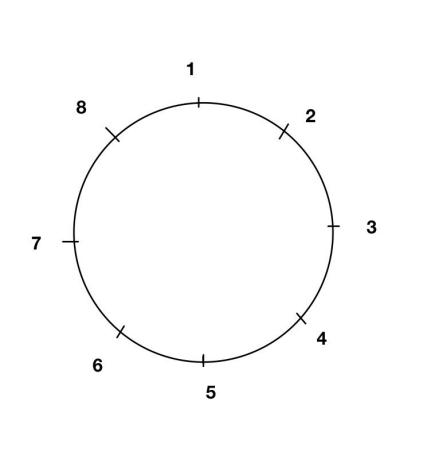
\includegraphics[width=.6\textwidth]{person}
    \caption{8名队员的位置与编号}
    \label{fig:p2}
\end{figure}
第一问中只要考虑1号和5号队员即可,其他人的合力是竖直向上的不会给鼓一个转动趋势,建立如图所示的空间直角坐标系
\begin{figure}[!h]
    \centering
    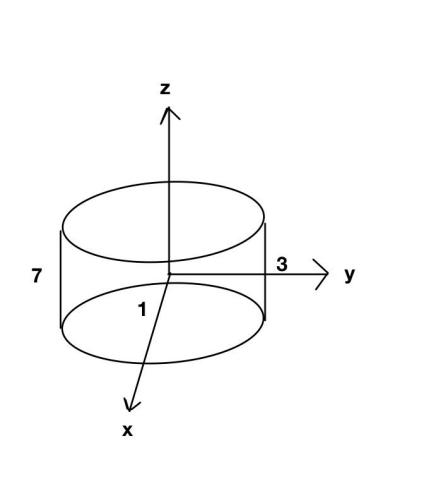
\includegraphics[width=.6\textwidth]{axes}
    \caption{8名队员的位置与编号}
    \label{fig:p3}
\end{figure}
列出力的矢量表达式,之后再用空间解析几何知识计算力臂,代入公式,易算得转动角度。
\end{enumerate}

\subsection{问题3}

在现实情形中,根据问题2的模型与计算,我们认为需要对问题1中给出的最优策略做出调整,调整如下:
\begin{enumerate}
\item 排球的跳动高度不能过高,弹起方向与鼓面法线的角度不能大于10°。以鼓面直径40cm计算,若鼓面不移动且排球弹起点为鼓面圆心,则当排球的弹起角度出现10°时倾斜时,当球的跳动高度为56.7cm时,球会落出鼓面。而要尽量使得球的跳动保持竖直状态,球与鼓面的接触点以落在距鼓面圆心20cm的范围内为最佳。这样算来,球在鼓面的跳动高度以60cm以内为好。
\item 尽量不要靠鼓面击打排球,只需要让球在水平的鼓面借助鼓面的弹性和排球的弹性自然跳动即可,只有当发现球的高度过低时才进行发力。这样可以减少发力次数,有利于发力效果更加稳定,并且使排球跳动高度不会过高。
\item 队员相互配合,尽量控制发力时间与发力大小一致。
\item 使得排球与鼓面接触位置稳定在距鼓面圆心20cm的范围内,当接触点偏离时,队员共同发力,调整位置,使接触点回归圆心。
\item 尽量保持鼓面水平,当鼓面出现倾斜使得排球偏移时,作出适当调整。
\end{enumerate}

\subsection{问题4}

\section{误差分析}

实际情况中,排球与鼓面都是粗糙的,之间存在摩擦力的作用,以及排球在碰撞时可能处于旋转状态等等,都会影响模型的精确程度。

假设已知排球与鼓面的摩擦系数$\mu$,我们按以下方式进行讨论,将碰撞前排球速度$v$分解为两个分量:垂直于鼓面的分量$v_\bot$;平行于鼓面的分量$v_\parallel$。将碰撞后的排球速度分量分别用$v'_\bot$和$v'_\parallel$来表示。排球与鼓面碰撞后,速度的垂直分量改变了自己的方向,而大小仍然未变。

为了证实这一点,我们对排球进行受力分析(如图)。垂直于鼓面的力$N$是由于排球形变产生的弹力,摩擦力为$f$,$N$与$f$夹角为$\gamma$。

排球与鼓面碰撞后的形变看作是弹性形变,碰撞后排球恢复了自己的形状,因而排球的弹性势能,在碰撞后重新变为排球的动能。换句话说,碰撞前后,排球沿鼓面法线方向运动的动能未变。而在摩擦力作用下,速度的平行分量发生了变化,摩擦力的方向与原平行分量的方向相反。如果排球与鼓面壁碰撞时不旋转,那么碰撞后的速度水平分量比$v_\parallel$小。这就是说,反射角$\beta$小于入射角$\alpha$,图1和图2所示的正是这样。如果碰撞前排球如图4所示方向旋转,当排球旋转得足够快时($\omega R>v_\parallel$),排球速度的水平分量向左,摩擦力的方向向右,并且速度的水平分量大于$v_\parallel$,这种情况下,反射角大于入射角。

另一种情况,当排球碰撞前不旋转,我们也认为,速度的水平分量不为零,在碰撞的过程中滑动并没有停止。弹力$N$是在球与鼓面接触时产生的,之后弹力$N$将逐渐增大,在排球形变达到最大程度时$N$达到最大值,此后$N$减小到零。在排球与鼓面碰撞过程中摩檫力$f$也不是常量,在任何时刻摩檫力的数学表达式为:
\begin{equation*}
	F_\textrm{摩}=\mu N
\end{equation*}
因此,在整个碰撞过程中,鼓面作用于球的合力的大小要改变,而方向不变。合力$Q$与鼓面法线的夹角为$\gamma$。由图3看出,$tan\gamma=\mu$,这样就有可能求出反射角。

根据牛顿第二定律,排球与鼓面碰撞时排球动量的变化量$\vartriangle P$与力$Q$同时产生。借肋于图2我们作出动量的变化量$\vartriangle P=m(v'-v)$(见图5)。
这个矢量与图3中的矢量$Q$一样,这个矢量与鼓面法线夹角为$\gamma$。由图5看出,
\begin{equation*}
	v'_\parallel=v_\parallel-2v_\bot tan\gamma
\end{equation*}
等式两端同除以$v_\bot$,并考虑到$\frac{v_\parallel}{v_\bot}=tan\alpha$,$\frac{v'_\parallel}{v'_\bot}=tan\beta$,$tan\gamma=\mu$,我们得到
\begin{equation*}
	tan\beta=tan\alpha-2\mu
\end{equation*}
一般而言,若排球碰撞前不旋转,则摩擦力会导致反射角小于入射角,由此可见摩擦力对模型精确程度确实有一定的影响。
\section{模型的优点与不足}
\subsection{模型的优点}
实际情况中,干扰因素可能有很多,条件也更复杂,我们对条件做了合理的假设与化简,适当舍去计算中的小量,从而使得计算难度相对降低,而模型拟合程度也较高。

在过程分析中,我们发现队员的发力点、所处的位置等条件,都会随机地发生一定的扰动,为了简化条件控制难度,我们将复杂的变量转化为用统一的物理量即发力的大小、角度等进行控制与表示,减少了模型所需的变量个数,从而降低了模型建立的难度与复杂程度。

在建立模型的过程中,通过视频资料,充分了解现实情况中,发力误差出现的来源。探究调整策略时,构造发力效果满足正态分布的随机数据,模拟现实情况中,队员发力时机和力度存在的误差,使得调整策略具有更稳定、更优良的实施效果。
\subsection{模型的不足}
短时间内空气阻力的影响可以忽略不计,但随着时间的延长,空气阻力的干扰程度逐渐增大,因此在建立长期模型时,还应将空气阻力纳入影响因素中。
\newpage

%参考文献
\begin{thebibliography}{9}%宽度9
    \bibitem[1]{liuhaiyang2013latex}
    刘海洋.
    \newblock \LaTeX {}入门\allowbreak[J].
    \newblock 电子工业出版社, 北京, 2013.
    \bibitem[2]{mathematical-modeling}
    全国大学生数学建模竞赛论文格式规范 (2019 年 9 月 12 日修改).
\end{thebibliography}


\end{document} 